\section{Model}
To reliably reproduce experimental observations of dynein's step, a model of dynein should responsibly conserve dynein's spatial information and complex structure without limiting the physical interactions with its environment. Doing so computationally introduces a strict balance between model accuracy and computational efficiency. In an attempt to best satisfy this difficult balance, we propose a simple model of dynein under a series of assumptions that benefits quick simulations of dynein taking a step. 


\subsection{2D Rigid Rod Model}
Since our goal is to investigate dynein's interhead coordination during its forward directed stepping, we decided to model dynein as a two-dimensional system of circular domains held together by massless rigid rods. These cirular domains embody the two binding domains, two motor domains, and one tail domain, where each domain act as independent angular springs with their own spring constants. A labeled picture of the model is shown below in Figure (\ref{fig:model}). 

\begin{figure}[H]
	\centering
	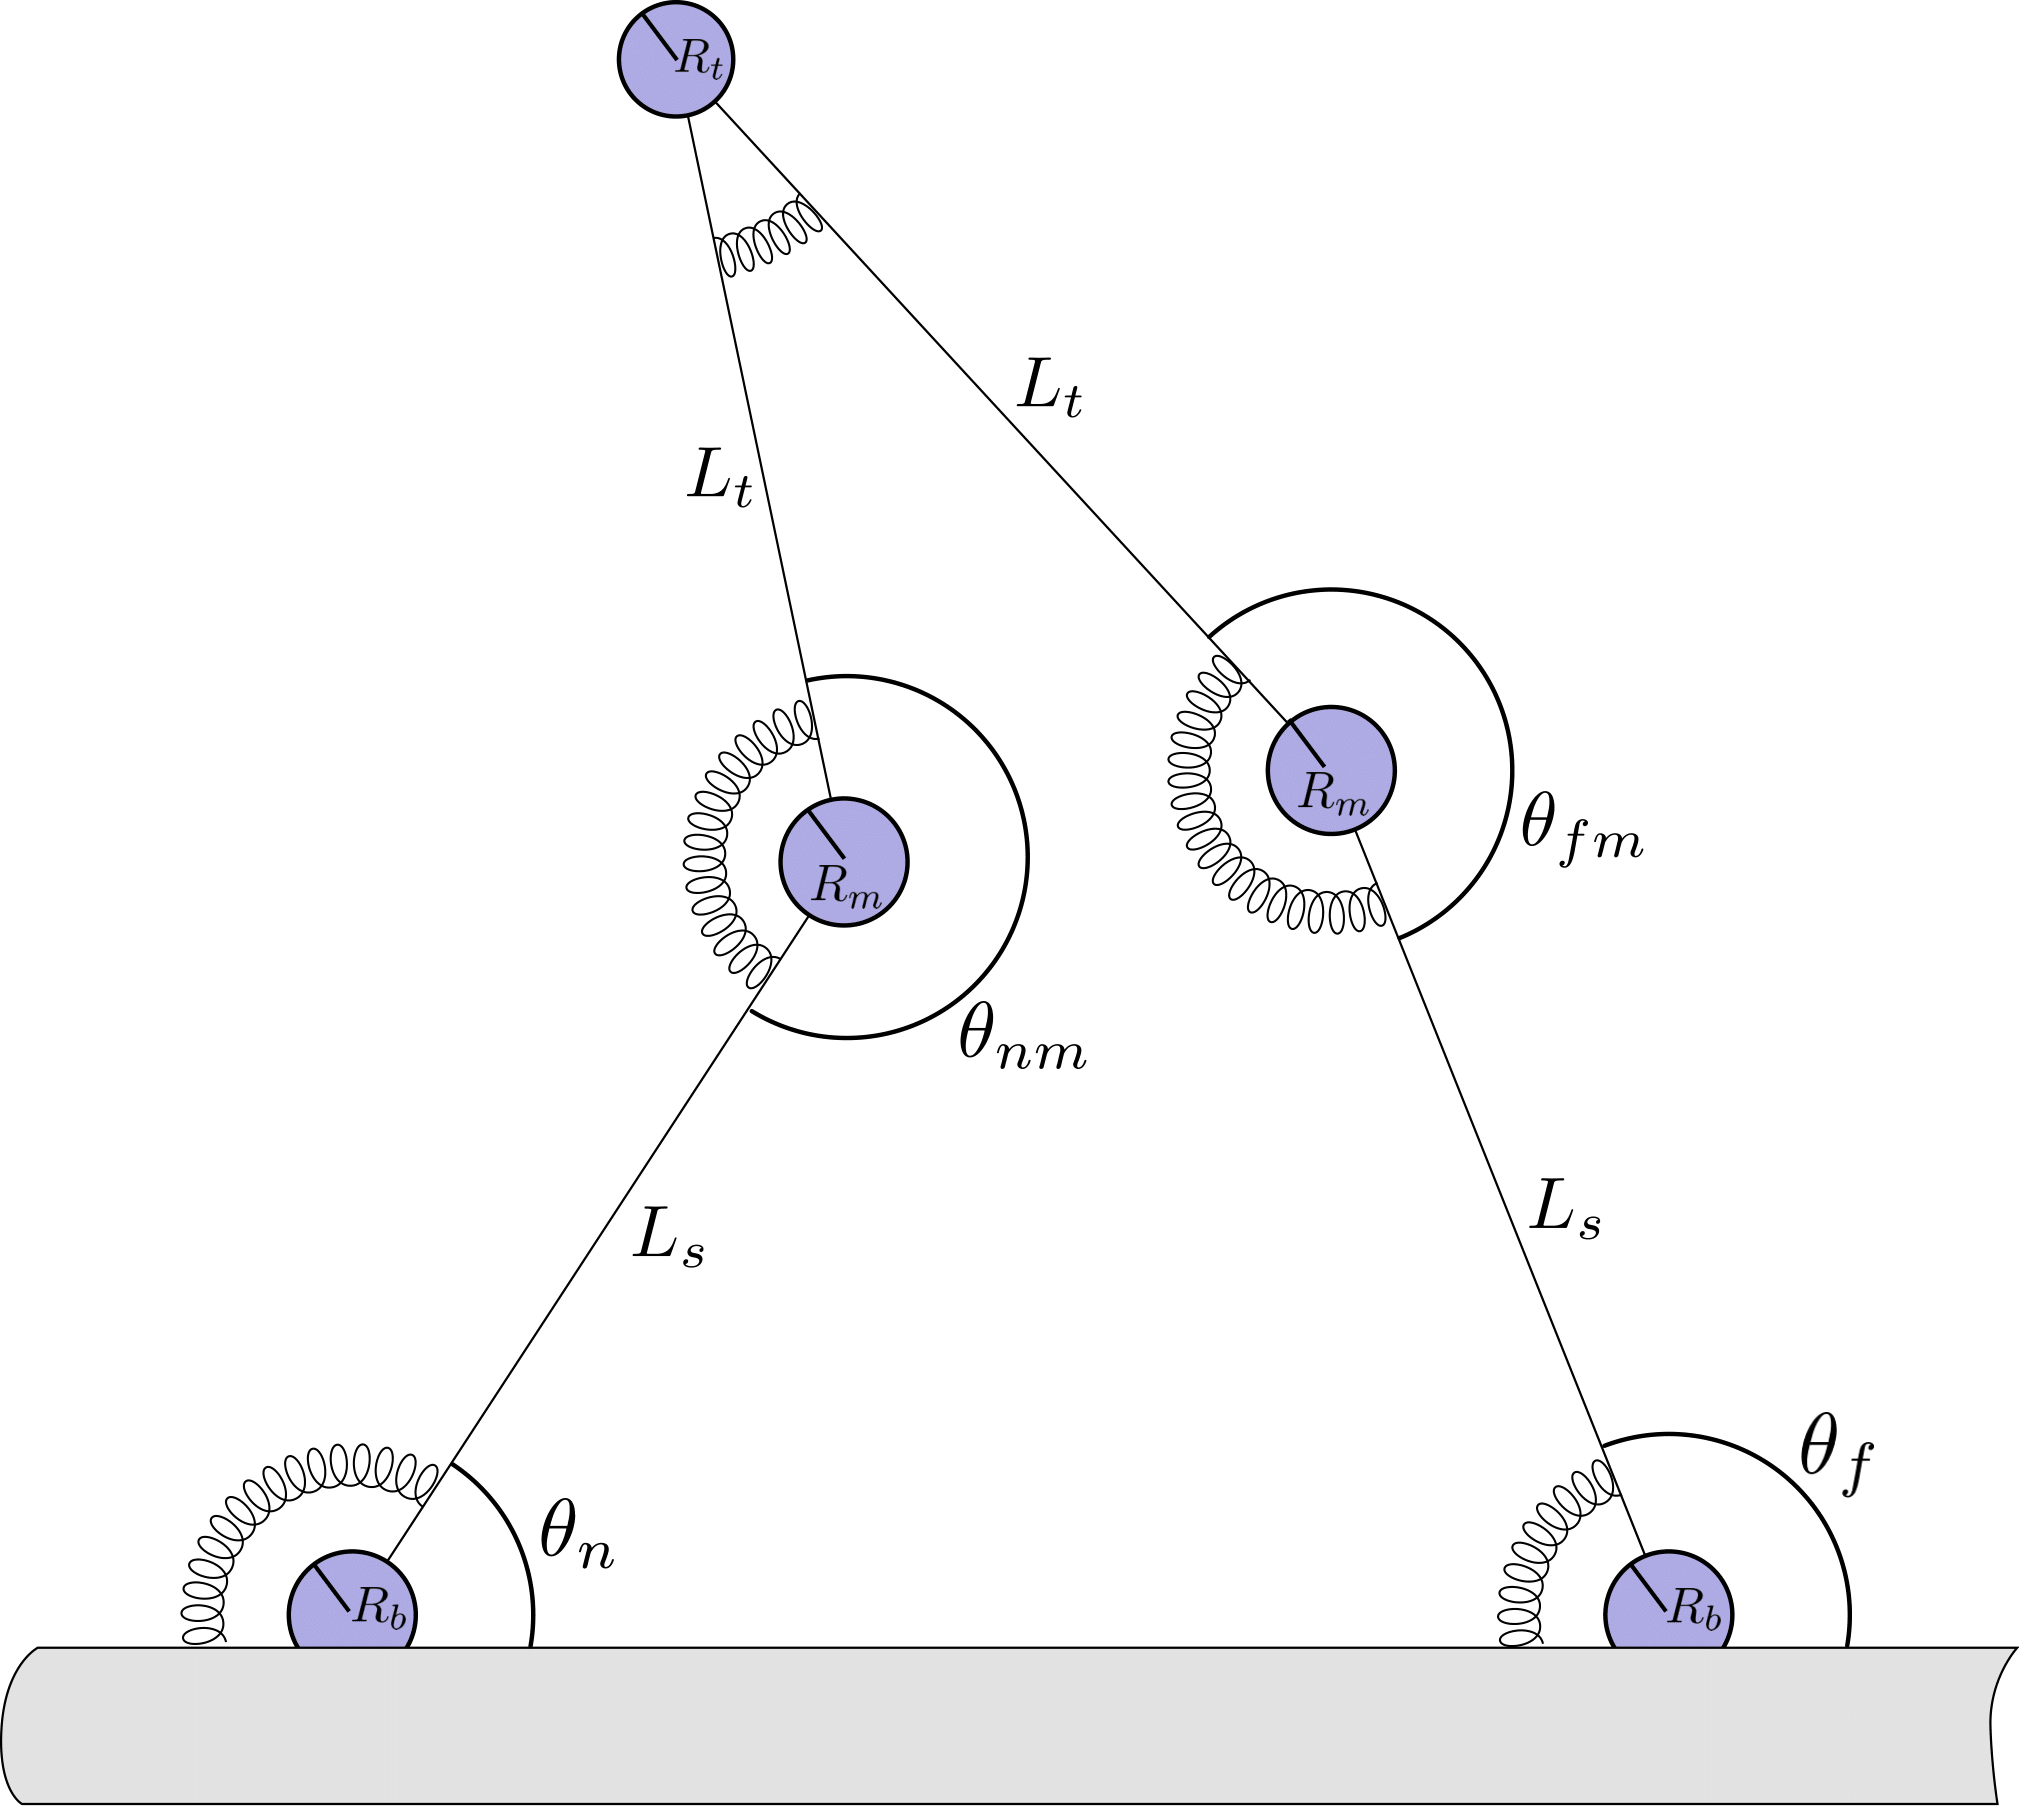
\includegraphics[width=0.6\columnwidth]{Figures/model-cartoon.png}
	\caption[Dynein Model]{\textbf{Dynein Model.} A model of the dynein in the both-bound state where both binding domains are bounded to the microtubule. The springs are only a visualization of how they control the domains and are not a part of the model geometry. \cite{Capek2017}}
	\label{fig:model}
\end{figure}

Despite dynein's step varying in both length and direction, we limit our model in one direction to eliminate the off-axis and only focus on dynein's forward stepping. This would simplify the asymmetry of the microtubule when dynein is stepping on the $\alpha$ or $\beta$ tubulin. We also assume massless stalks and linkers due to the strong drag force terms dominating the mass of the rods and domains in the equations of motion. The reasoning for this will be later discussed in Section \ref{sec:BrownianDynamics} when we introduce Brownian dynamics. Although the stalk and linker of real dynein definitely have mass, we counteract the loss of interactions the rods experience with the environment by increasing the radii of the domains abitrarily 10\% larger than experimental measurements.

\subsection{Domains as Angular Springs}
To best simulate the stretching and forward kicking motion of the power stroke, we define the domains to act as springs with spring constants $c_b$, $c_m$, and $c_t$. This is analogous to how humans walk, where the domains correspond to flexible joints when taking a step. Defining the domains as springs influences forward bias walking by introducing a restoring force in each domain using Hooke's law, 
\begin{equation}
    F_i=-c_i(\theta_i-\theta_{i,eq}),
\end{equation}
where $c_i$ is the spring constant, $\theta_i$ is angle corresponding to the $i^{th}$ domain, and $\theta_{i,eq}$ is the equilibrium angle in which biases the motion. Using this, we can calculate the energy of each domain by integrating and arriving to the familiar equation for spring energy:
\begin{equation} \label{eqn:energy}
    U_i=\frac{1}{2}c_i(\theta_i-\theta_{i,eq})^2.
\end{equation}
%Since dynein is symmetric for each heavy chain leg, the equilibrium angle will be identical for both binding and motor domain pairs, i.e. $\theta_{b,eq}$ is defined as the equilibrium angle for both binding domains, while $\theta_{m,eq}$ is defined as the equilibrium angle for both motor domains. 
This equation is used throughout the simulation to determine the total energy of our dynein at a given conformation. 


\subsection{Two-State System}
According to the mechanochemical cycle (Figure \ref{fig:MechanochemicalCycle}), dynein can be in eight states over the course of a single step. However, many of these states possess similar conformations, where the dynein either has low affinity (unbinded domain diffusing above microtubule) or high affinity. Since we assume simple ATP exchange and that the two physical states are during binding and unbinding, we categorize the cycle into two main conformations: the pre-stroke one-bound state and the post-stroke both-bound state.

\begin{figure}[H]
	\centering
	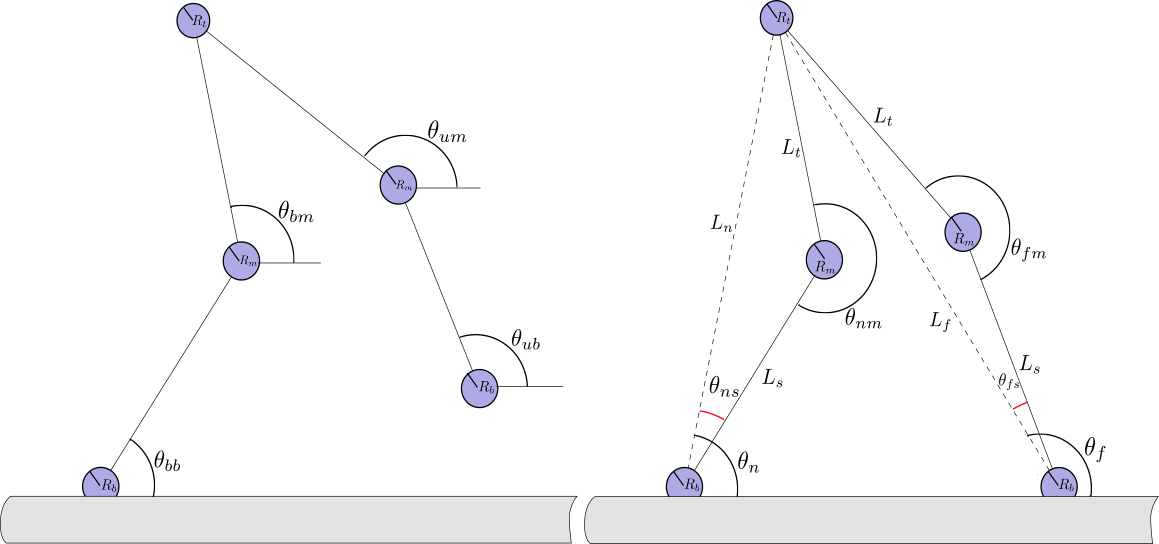
\includegraphics[width=0.9\columnwidth]{Figures/OB_vs_BB.PNG}
	\caption[One-Bound vs. Both-Bound]{\textbf{One-Bound vs. Both-Bound} \textit{Left}: Prestroke one-bound state with labeling scheme 'b-’ and ‘u-’ for bound leg and unbound leg. \textit{Right}: Poststroke both-bound state with labeling scheme ‘n-’ and ‘f-’ for ``near" leg and ``far'' leg. \cite{Capek2017}.}
	\label{fig:OBvsBB}
\end{figure}

Differentiating the two conveniently biases the conformational changes by defining different equilibrium angles for both states. Since dynein is symmetric for each heavy chain leg, the equilibrium angles for the both-bound state is identical for both binding and motor domain pairs, i.e. $\theta_{b,eq}$ is defined as the equilibrium angle for both binding domains, while $\theta_{m,eq}$ is defined as the equilibrium angle for both motor domains. However, in the one-bound state, the unbound leg exhibits the powerstroke and kicks out. Therefore, the equilibrium angles for the motor domains differ in order to bias the unbound leg to straighten and perform the powerstroke. This straightening mechanic resembles the linker being primed before allowing the binding domain to rebind.


\subsection{Transitioning Between States}
%\textit{Physics about conformational energy changes. How we model transitioning between BB state and OB state using transitioning rates and spring energies.}

Similar to other simulations, the binding and unbinding process is governed by rate-limiting steps, where each process is associated with binding rates. These binding rates are model parameters defined by binding constants with units of probability per time. When the dynein is in the one-bound state, the binding domain depends on two rebinding parameters: the affinity transition time ($t_a$) and the binding rate ($\rho_b$). We assume that the one-bound can only bind when high affinity completely transitions into low affinity and when the domain is within a vertical range of the microtubule, i.e.
\begin{equation}
	t>t_a=\frac{1}{k_a}
\end{equation}
and
\begin{equation}
	\rho_b=k_b(1-H(r_{ub,y}-\epsilon)).
\end{equation} 
Here, $t$ is the total one-bound time, $k_a$ is the affinity transition rate, $k_b$ is the binding rate constant, $H$ is the Heaviside step function, $r_{ub,y}$ is the y position of the unbound binding domain, and $\epsilon$ is the range within the microtubule.

When the dynein is in the both-bound state and wants to unbind, we incorporate a stepping bias in the unbinding rate. As supported from Yildiz in Figure (\ref{fig:trailingbias}), the likelihood of the trailing leg unbinding is greater than the leading leg when the distance between the two legs increases. 


\begin{figure}[H]
	\centering
	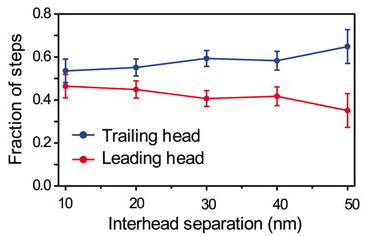
\includegraphics[width=0.6\columnwidth]{Figures/trailingbias.png}
	\caption[Probability of Unbinding Bias]{\textbf{Probability of Unbinding Bias.} The probability of either trailing or leading steps which correspond to the model's ``near" or ``far" leg unbinding, respectively. \cite{Dewitt2012}.}
	\label{fig:trailingbias}
\end{figure}

To favor trailing steps, we define an angle dependent exponential factor within the binding domains and mathematically express this as,
\begin{equation}
	\rho_{ub}=k_{ub}e^{C(\theta_b-\theta_{b,eq})}.
\end{equation}
We introduce a new model parameter $C$, the exponential unbinding constant, that controls this bias. To achieve trailing step bias, we define $C$ to be negative because the trailing $\theta_b$ tends to be less than the leading $\theta_b$ and  when $\theta_b$ is less than $\theta_{b,eq}$, the unbinding rate becomes large.


\section{Simulation}

The key difference between the works in \cite{Capek2017, waczak2019drunken} and this paper is the implementation of a Monte Carlo algorithm in replacement for the Brownian dynamics both-bound state. In addition to the large both-bound time mentioned earlier, they noticed that the initial both-bound configuration of the motor and tail domains do not impact the stepping, giving a better incentive to apply a Monte Carlo approach. This new method of analyzing the both-bound state will significantly improve computational efficiency while still maintaining the dynamical simulation of the actual step in the one-bound state. 

%These quick simulations are governed by a Monte Carlo algorithm, while the movement of the model is dictated by equations of motion describing domains interacting with a force of drag and a random force. This type of molecular simulations are more commonly known as Brownian dynamics. (\textbf{Possible take out sentence introducing MC and Brownian dynamics for later})


\subsection{Brownian Dynamics for One-Bound}
\label{sec:BrownianDynamics}

When simulating dynein's one-bound motion, the domains of constant mass must obey classical Newtonian physics and follow Newton's laws of motion. That is,
\begin{equation}
	\sum_{i}\textbf{F}_i=m\ddot{\textbf{r}}.
\end{equation} 
For the domains in the aqueous environment of the cell, linear drag force is
\begin{equation}
	\textbf{F}_{drag}=-\gamma \dot{\textbf{r}},
\end{equation}
where $\gamma$ is the drag coefficient defined by Stokes' law,
\begin{equation}
	\gamma=6\pi\eta a.
\end{equation}
This equation specifies the drag term by a given radius $a$ and liquid viscocity $\eta$. 

A second force is the random force inspiring the Brownian motion. \textbf{F}$_{rand}$ describes the random interactions between the domains and the solvent paticles. \textbf{F}$_{rand}$ is sampled from a zero-centered Gaussian with variance
\begin{equation}
	\sigma^2=\sqrt{\frac{2\gamma}{\beta\Delta t}},
\end{equation}
where $\beta=\frac{1}{k_bT}$  and $\Delta t$ is a time-step. 

The final force is the tension force, \textbf{F}$_T$, between the domains \textit{via} their connecting rods. Incorporting all these forces, we produce the \textit{Langevin Equation}:
\begin{equation}
	-\gamma \dot{\textbf{r}} + \textbf{F}_{rand} + \textbf{F}_T = m\ddot{\textbf{r}}.
\end{equation}
To properly demonstrate Brownian dynamics, we must assume strong drag where $|\gamma \dot{\textbf{r}}|\ll |m\ddot{\textbf{r}}|$. In other words, we assume that the immense viscosity in the environment restricts the ability for the domains to accelerate. Simplifying the \textit{Langevin Equation} and solving for $\dot{\textbf{r}}$, we get:
\begin{equation}
	\dot{\textbf{r}}=\frac{1}{\gamma}(\textbf{F}_{rand} + \textbf{F}_T)
\end{equation}
which is a differential equation we can solve for the equations of motion for the domains in the one-bound state. The derivation and final equations of motion can be found in \cite{Capek2017}


\subsection{Monte Carlo for Both-Bound}
Since dynein spends most of its stepping time in the both-bound state, we safely assume dynein equilibriates before unbinding. This allows us to use Monte Carlo methods for analyzing dynein's step by interpreting our model as a system. Typically, Monte Carlo methods analyze equilibrium theromodynamics of fluids, where a system of atoms possess many different microstates \cite{lim2007vorticity}. For this model, dynein is the system and the many possible both-bound configurations are the ``microstates." However, unlike the more commonly known Markov Chain Monte Carlo, each both-bound configuration is independent and can generate different total energy values. This produces a large ensemble of of both-bound configurations, which we sample to create stepping statistics. Eventually, these statistics will reduce to probability distributions for important variables.

With the assumption of thermodyamic equilibrium during the both-bound state, we use a Boltzmann distribution to define the probability of a configuration and calculate the relative unbinding probability with a proportionality expression. That is, 
\begin{equation}
	P_{ub}\propto e^{-\beta E_{total}}.
\end{equation}
With this Boltzmann factor, we can also generate a partition function, 
\begin{equation} \label{eqn:partition}
	Z=\sum_{i}e^{-\beta E_{total,i}},
\end{equation}
where $i$ refers to the specific both-bound configuration. In order to guarantee an accurate thermodynamic ensemble of both-bound configurations, the simulation must run a large number of trials to ensure that the sample space is covered well. The thermodynamic ensemble then generates an ensemble of steps that can eventually produce smooth statictics. With the partition function defined in Equation (\ref{eqn:partition}), we also define ensemble averages for both-bound statistics, such as the average unbinding rates, unbinding probability, and both-bound time. The equations to do so are all shown below in that order:
\begin{equation}
	\langle\rho_{\textit{ub, trail.}}\rangle=\frac{\sum_{i}\rho_{\textit{ub, trail.}} e^{-\beta E_{total,i}}}{Z}, \indent \langle\rho_{\textit{ub, lead.}}\rangle=\frac{\sum_{i}\rho_{\textit{ub, lead.}} e^{-\beta E_{total,i}}}{Z}
\end{equation}
\begin{equation} \label{eqn:ProbTrail}
	\langle P_{\textit{ub, trail.}}(L)\rangle = \frac{\langle\rho_{\textit{ub, trail.}}\rangle}{\langle\rho_{\textit{ub, trail.}}\rangle + \langle\rho_{\textit{ub, lead.}}\rangle}
\end{equation}
\begin{equation}
	\langle t_{bb}(L) \rangle =\frac{1}{\langle\rho_{\textit{ub, trail.}}\rangle + \langle\rho_{\textit{ub, lead.}}\rangle},
\end{equation}
where $trail.$ and $lead.$ signifies a trailing or leading step.



%\textit{STRAIGHT FROM PROPOSAL. FIXME}

%Our entire model of dynein will be coded with a combination of both Python and C++. The structural features of dynein will be captured with a two-dimensional geometric model of circular domains connected by rigid rods. The dynamics of dynein will be captured by imposing both equilibrium and Brownian forces on each circular domain of the model, while the chemical properties will be modeled by sporadically transitioning between two states: a poststroke both bound state, and a prestroke one bound state. These two states are shown below in Figure 2.
%
%The simulation for stepping will consist of running multiple independent steps that starts in a both bound configuration and transitions into the Brownian dynamics one bound state. In this state, each domain will undergo Brownian forces until the unbounded leg diffuses back onto the microtubule, thus completing a step. The Brownian dynamics only affects the one bound state since that is the only time (in our model) the domains undergo molecular interaction with its surroundings to achieve processive motion. This Monte Carlo method of collecting an ensemble of statistics after many simulations will lead to probability distributions of measured variables that can be compared with experimental results. The common experimental results analyzed in this field are the distribution of step lengths (defined as the final displacement of the “stepping” leg minus the initial displacement), stepping times, probability of the binding domain unbinding, and the velocity of a step. Once sufficient data is collected for each listed variable, plotting scripts on Python will be used to visualize the possible relationships between these variables and generate analysis for our model’s stepping patterns. Currently, a paper published by Dr. Ahmet Yildiz from the University of Berkeley proposed a possible relationship within dynein’s stepping, implying inter-step correlation [3]. Our model aims to reproduce these results by finding a set of parameters that matches Yildiz’s observation in the form of a linear regression of the step lengths against the initial binding domain separation. We hope to either support Yildiz’s claim or infer some new property of dynein that generated Yildiz’s observation.